\chapter{Designing an Extensible Tool for Object-Centric Process Mining}
\label{chap:design}

Building on the requirements defined in the previous chapter (\autoref{tab:requirements}), this chapter proposes the architecture and design of a framework intended to address them.

Requirements \req{BF-2a} and \req{BF-2b} call for a graphical user interface that adapts to different display sizes and maintains a consistent appearance across operating systems.
To satisfy these requirements, we propose implementing the framework as a web application.
This allows the user interface to be rendered in the browser, enabling consistent behavior across operating systems and supporting cross-platform compatibility.
In addition to running locally, the web application can also be hosted as an additional deployment option, further reducing dependencies and simplifying setup (\req{BF-5b}, \req{BF-5c}).
Figure~\ref{fig:ocelescope-architecture} provides an overview of the proposed system architecture.

\begin{figure}[ht]
	\centering
	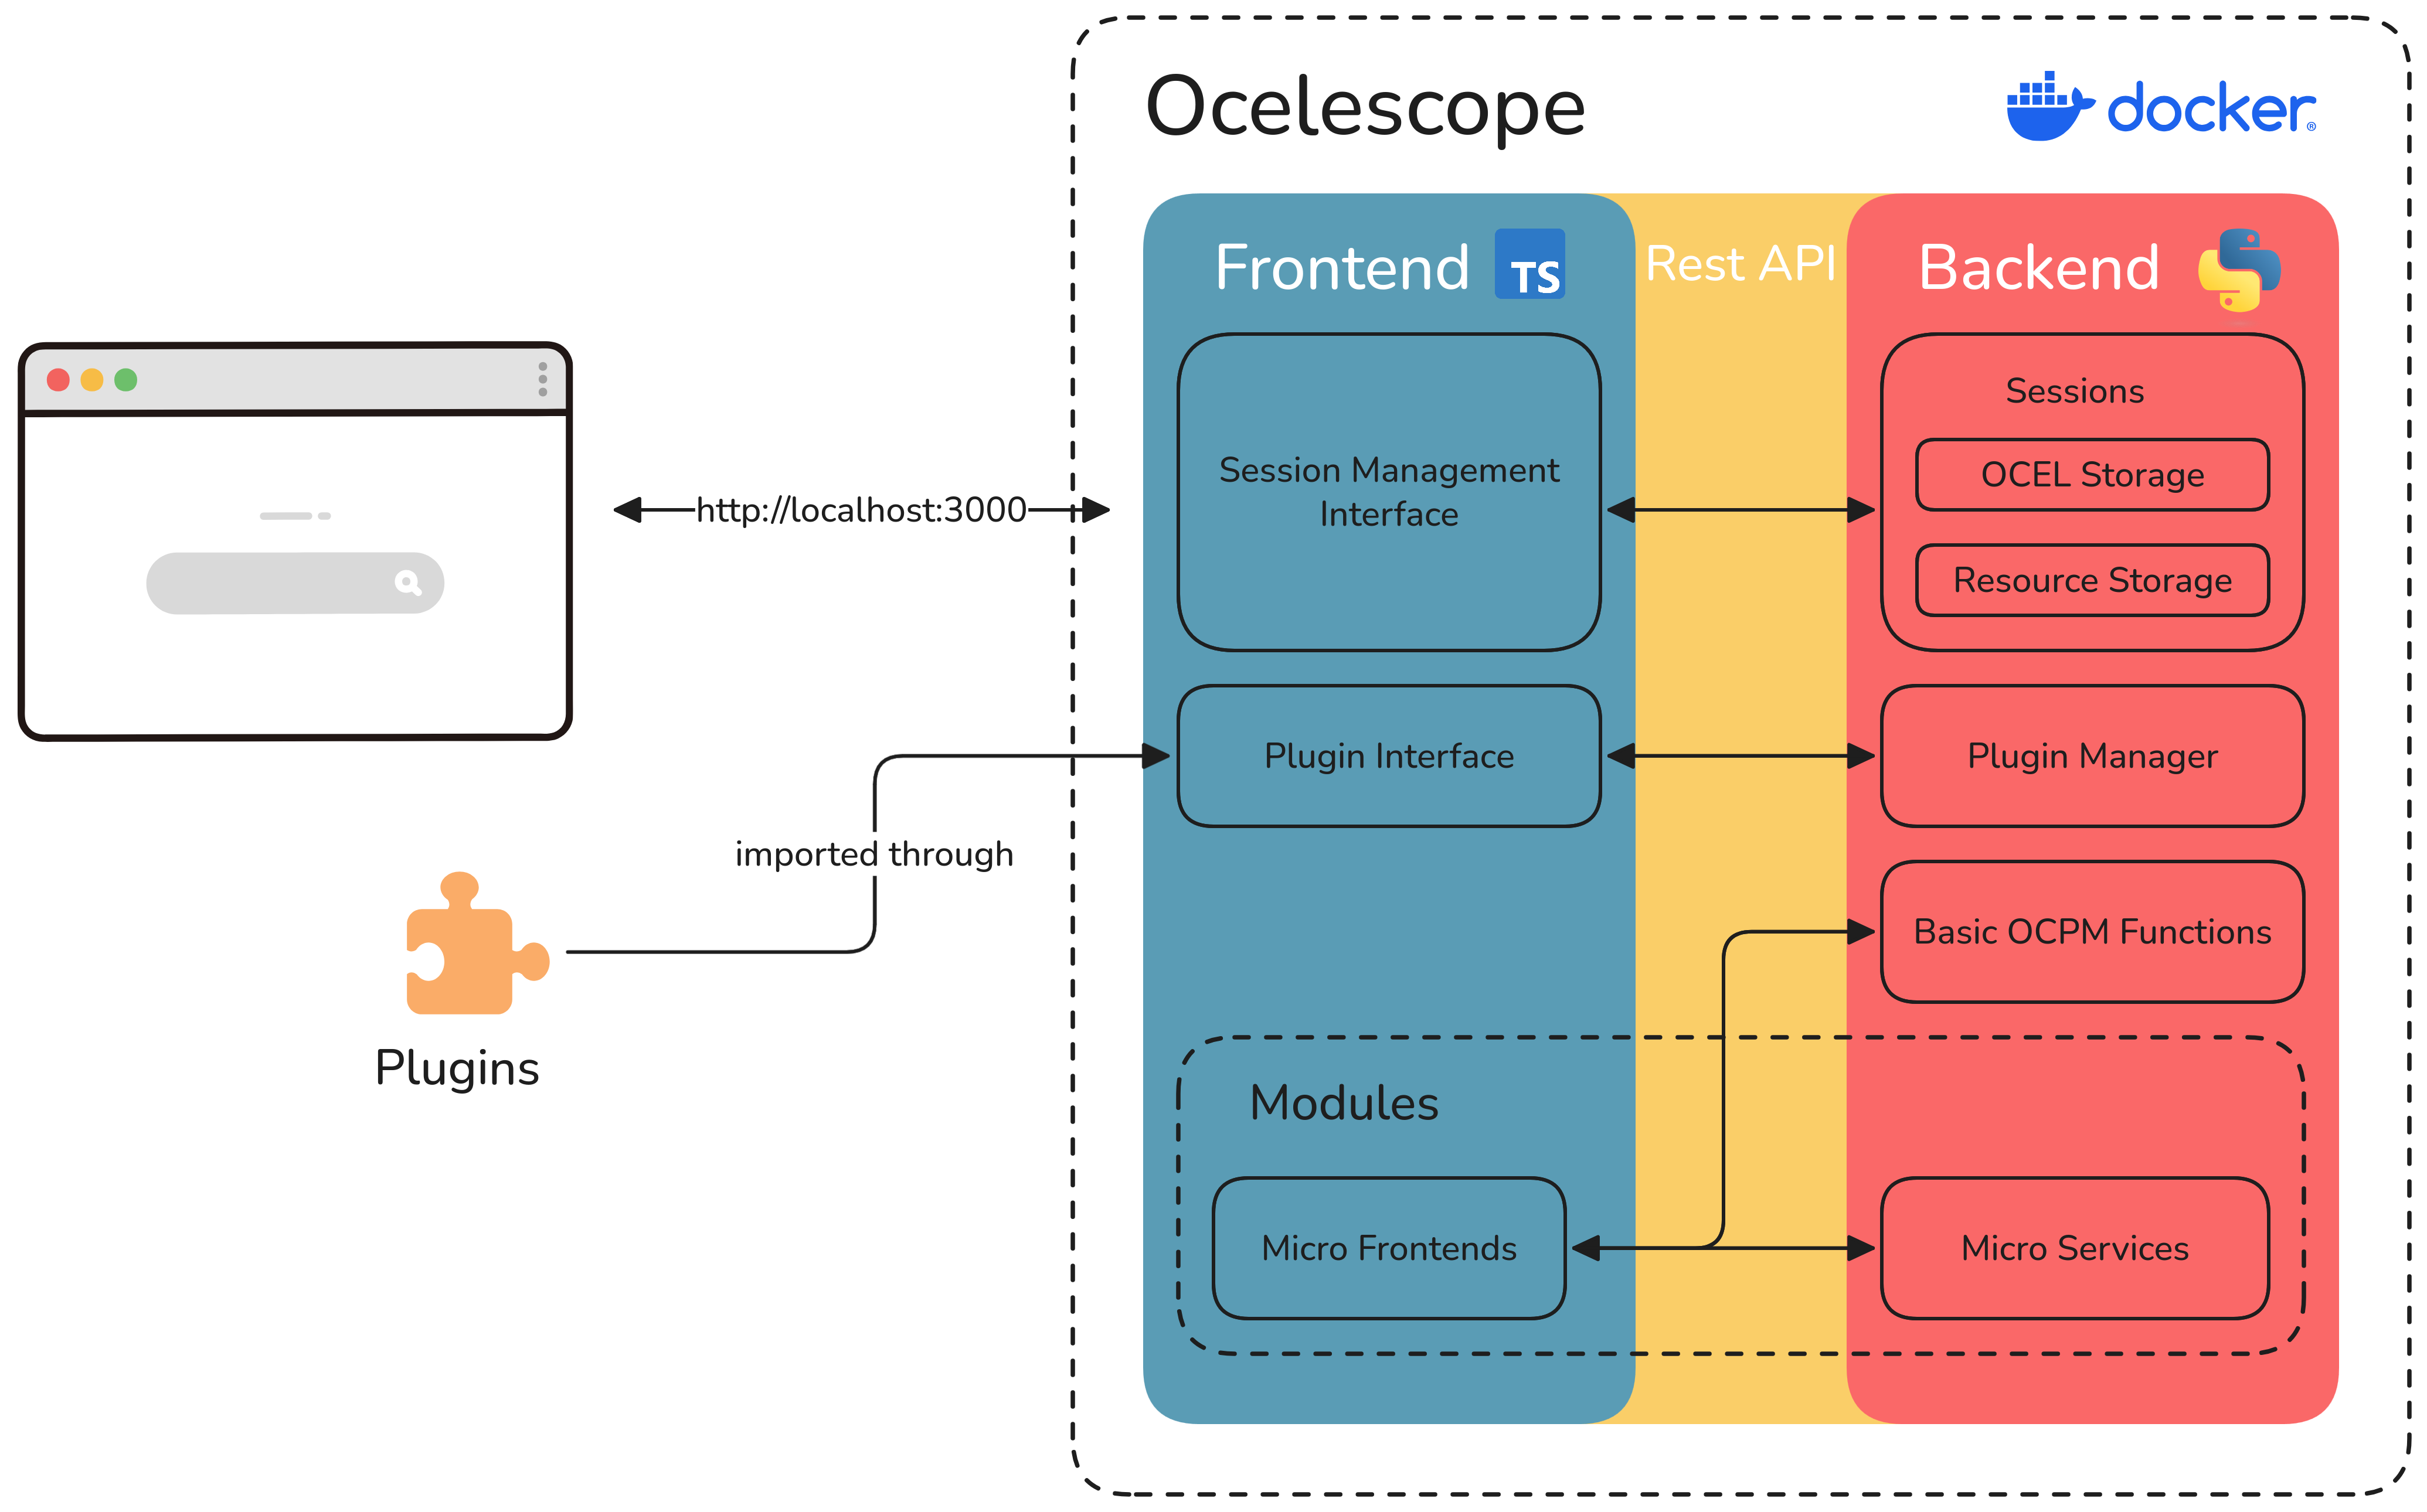
\includegraphics[width=0.75\textwidth]{figures/design/Architecture.png}
	\caption{Overall architecture of the Ocelescope framework, showing the separation of frontend and backend, the REST API boundary, and the roles of plugins and modules.}
	\label{fig:ocelescope-architecture}
\end{figure}

To support this design, the framework follows a \textbf{frontend--backend} architecture.
The frontend provides the graphical user interface through which users interact with the framework.
Requirements \req{EM-1} and \req{EM-4a} call for implementing the user interface using established web frameworks and adhering to their implementation styles.
We therefore propose implementing the frontend in TypeScript, which supports the use of established frontend frameworks and aligns with the technology stacks of existing OCPM tools such as OCPQ~\cite{ocpq} and ProAct~\cite{proact}.

Both external and embedded extensions should be able to implement process mining functionality in Python (\req{EX-6}, \req{EM-2}).
Although OCPM functionality can run in the browser, for instance via WebAssembly as demonstrated in \textit{Rust4PM}~\cite{rust4pm}, this is not ideal for Python-based extensions because Python-to-WebAssembly tooling is still limited in package support and often introduces additional complexity.
We therefore propose implementing the backend in Python, which enables extensions to execute process mining functionality natively.

To support OCEL management, the backend provides functionality for importing and exporting logs in standard OCEL formats (\req{BF-1a}).
To allow multiple users to work on the same \textit{Ocelescope} instance independently, particularly in a hosted deployment, the backend assigns each user to a separate session.
A session stores the imported OCELs and the OCPM artifacts produced by external extensions.
Communication between the frontend and the backend is handled through a REST API.

To support the implementation of embedded and external extensions, the framework adopts architectural patterns introduced in \cref{chap:prelim}.
External extensions follow the \textbf{plugin architecture}, while embedded extensions follow the \textbf{microservice architecture} and the \textbf{microfrontend architecture}.
Their design and use within the framework are discussed in the following sections.

\section{Plugin Architecture}

To support external extensions that integrate into the main interface without recompilation or restart (\req{EX-1}) while introducing only minimal additional abstractions for developers (\req{EX-5}), \textit{Ocelescope} follows a plugin architecture.
As introduced in \cref{chap:prelim}, plugins are implemented by providing a plugin interface, also known as the plugin contract.
In this section, we describe the structure of the implemented plugins.

Plugins in Ocelescope consist of four main building blocks:

\begin{enumerate}
	\item \textbf{Metadata}, which provides basic information about the plugin and is used by the frontend.
	\item \textbf{Resource definitions}, which specify custom OCPM artifacts that can be used as input or output of plugin functions.
	\item \textbf{OCEL extensions}, which define extensions of the OCEL~2.0 format and allow OCELs to be enriched with additional metadata.
	\item \textbf{OCPM functions}, which implement the actual process mining logic and form the main functional part of the plugin.
\end{enumerate}

In the following sections, we describe these building blocks in detail.

\subsection{Resource Definitions}

Resources in \textit{Ocelescope} define custom OCPM artefacts and build on the resource concept used in ProM.
Resources in \textit{Ocelescope} represent entities that are not OCELs but are still exchanged between functions or serve as intermediate results. Typical examples include process models such as Petri nets or directly follows graphs, as well as analysis results like those produced by ProAct~\cite{proact}.

When a plugin is loaded, all resources it defines are registered automatically in the framework. Each resource consists of three main components:
\begin{enumerate}
	\item \textbf{Metadata:} A name and a description used for presentation in the user interface.
	\item \textbf{Schema definition:} A JSON Schema that describes the structure of the resource instances.
	\item \textbf{Visualization function (optional):} A function that maps a resource instance to one of the predefined visualization data structures in the framework.
\end{enumerate}

\begin{figure}[ht]
	\centering
	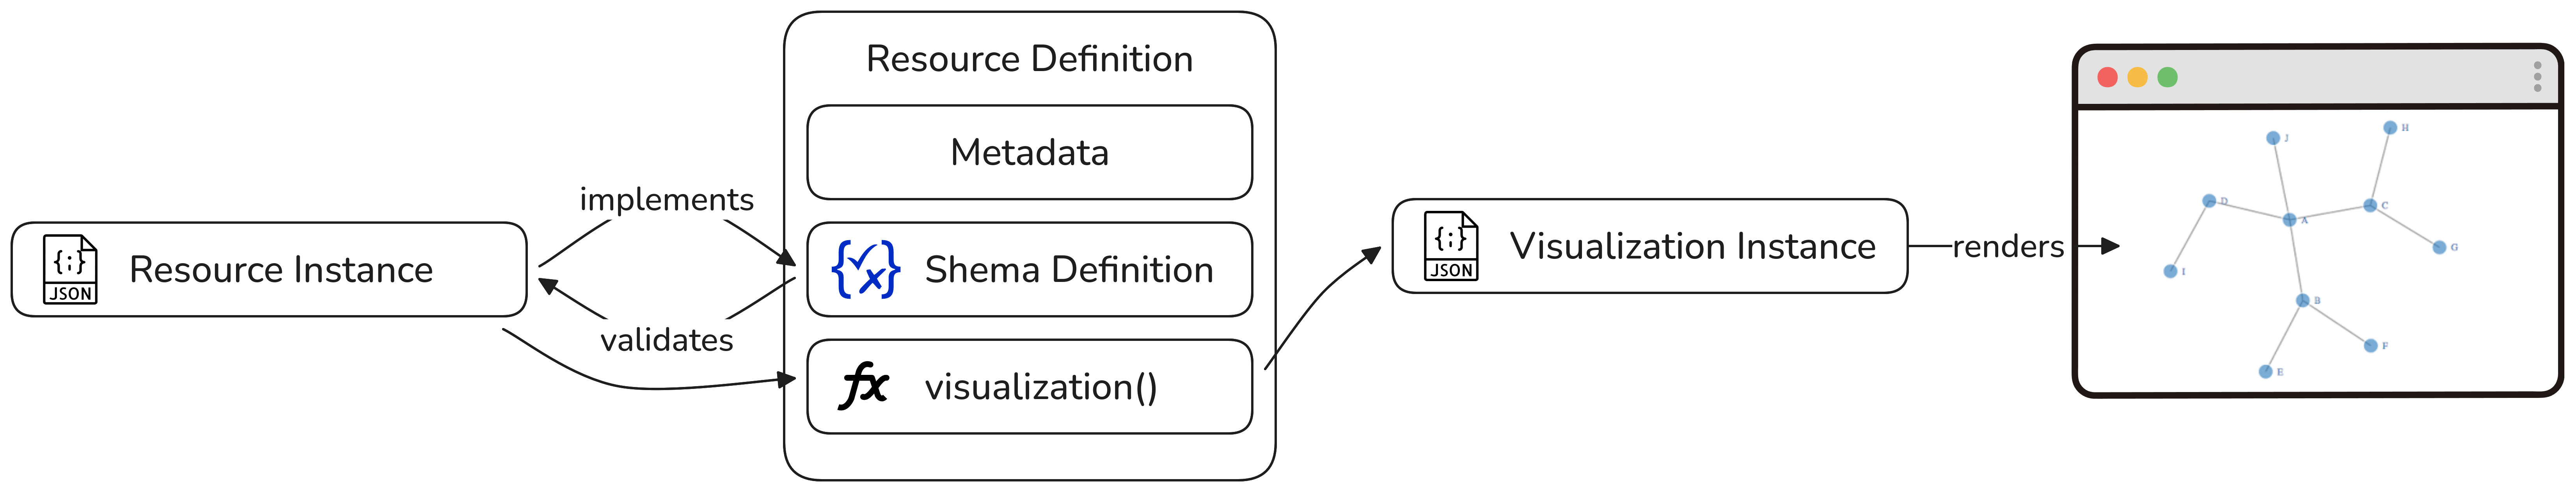
\includegraphics[width=0.95\textwidth]{figures/design/Resource Overview.png}
	\caption{Overview of a resource definition and its use. A resource instance must conform to its JSON schema, and an optional visualization function maps the instance to a visualization that can be rendered in the frontend.}
	\label{fig:resource-overview}
\end{figure}

Using JSON Schema to define resources automatically defines an exchange format (\req{EX-2a}) that allows them to be exported, shared, and reimported across different \textit{Ocelescope} instances.
Resources should also be compatible across plugins (\req{EX-2b}).
For example, a Petri net discovered by one plugin should be usable as input for another plugin that performs conformance checking.
\textit{Ocelescope} supports this through two mechanisms:

\begin{enumerate}
	\item \textbf{Common resource models:} Frequently used artefacts, such as Petri nets or directly follows graphs, are provided as predefined resource definitions.
	\item \textbf{Schema hashing:} During registration, each JSON Schema is hashed. Resources with identical hashes are treated as equivalent. This also allows support for new or niche artefacts, such as TOTeM~\cite{totem}, to be used in multiple plugins without changes to the core framework.
\end{enumerate}

In addition, resources can optionally provide visualization functions that map a resource instance to a predefined data structure, for which a corresponding viewer is implemented in the frontend (\req{EX-3a}).
This follows a common approach in extensible tools: ProM resources can define visualizers that appear in the View tab, and KNIME nodes can provide optional \texttt{NodeView} implementations.
Restricting resources to a predefined set of visualization types simplifies development, but it also requires the framework to support a sufficient number of common visualization types.

Resources must also support nesting and annotations (\req{EX-2c}).
One possible approach would be to define a separate resource type for each annotated variant of a model. However, this would break compatibility.
For example, a Petri net annotated with token-based replay results should still be usable as a standard Petri net.

For this reason, resources in \textit{Ocelescope} can be composed of other resources. The standard Petri net resource definition includes generic annotation fields for arcs, transitions, and places. These fields can store JSON data that represents instances of other resources. The same principle applies to visualization data structures. A graph visualization, for example, can embed tables or charts within its nodes or edges, which enables hybrid representations (\req{EX-3b}).

This design allows the creation of composite resource instances and visualizations. A Petri net annotated with performance data, similar to the models used in OPerA~\cite{opera}, can therefore be represented as a graph with nested visualizations for each element.

\subsection{OCEL Extension Definitions}

OCEL extensions are used to embed domain-specific data into OCELs (\req{BF-1b}).
For instance, in \cite{qrpm}, OCELs are enriched with item counts to support OCPM techniques specific to logistic processes.
Extending the \textit{OCEL 2.0} standard is not reasonable in this case because item counts are only relevant for logistic processes.
Extending the standard every time a domain requests additional data would increase its size without a tangible benefit.
Creating a new OCEL format would introduce compatibility issues with existing OCPM tools, making it difficult to apply standard OCPM techniques.

\textit{Ocelescope} therefore allows plugins to define OCEL extensions. These extensions enable plugins to embed additional data directly into OCELs using their native file formats. For example, OCEL files in JSON format can be extended with additional fields. This approach preserves the validity of the OCEL files and keeps the extended data closely integrated with the log.

In Ocelescope an extension defines three functions:
\begin{itemize}
	\item \textbf{Check:} Checks if an OCEL file contains extension data.
	\item \textbf{Import:} Extracts the extension data from the OCEL file and creates an extension instance that can be used in plugin functions.
	\item \textbf{Export:} Embeds an extension instance into an OCEL file.
\end{itemize}

These extension definitions are stored in a registry in the backend. When an OCEL is imported, the backend evaluates all registered extensions using their check functions. Extensions that apply to the file extract their associated data and attach it to the corresponding OCEL instance. When the file is exported, the attached extension data is written back into the OCEL file using the corresponding export functions.

\subsection{Plugin Functions}

Plugins in \textit{Ocelescope} can provide multiple process mining functions that run in the \textit{Ocelescope} environment.
A plugin function is an object-centric process mining operation written in Python with a clearly defined input and output (\req{EX-6}).
This input and output based definition follows established patterns from other process mining tools, such as ProM actions or KNIME nodes.

\subsubsection{Input Definitions}

Input definitions specify the parameters of a plugin function and are also used to generate the input user interface automatically.
A plugin function may define \textbf{OCEL inputs}, \textbf{resource inputs}, as well as additional \textbf{configuration inputs}.

Each OCEL and resource input is assigned a unique parameter name that identifies it within the function. OCEL inputs may also declare required OCEL extensions that must be present for the function to be executed.

Configuration inputs cover all remaining parameters that are neither OCELs nor resources. Typical examples include numeric thresholds, text-based filters, or boolean options that influence the computation. This is comparable to the input mechanisms used in KNIME’s \texttt{NodeDialog} or the user-configurable parameters of ProM actions.

In addition to static configuration inputs, some fields must be populated based on the values of other inputs. For example, an input field may need to list available activities, object types, or attribute names derived from the selected OCEL. To support such cases within the same input definition based on configuration files, \textit{Ocelescope} provides two mechanisms for extending configuration fields:

\begin{itemize}
	\item \textbf{OCEL-dependent fields:} Fields whose values are derived from a selected OCEL input. These fields reference the parameter name of an OCEL input and specify the type of data to extract, such as activity names or object types.
	\item \textbf{Computed fields:} Fields whose values are generated dynamically by a callback function that receives the current form state. This enables context-dependent input options while preserving the same input definition structure.
\end{itemize}

All plugin inputs are defined using JSON Schema. As discussed in \cref{chap:prelim}, JSON Schema is commonly used to define and validate inputs in REST APIs and is well suited for defining complex input definitions. The input user interface is generated automatically from the schema without additional development effort.

OCEL and resource fields are populated with all matching OCELs and resources that are currently available in the session. OCEL-dependent fields and computed fields are populated automatically based on the current input state.

This approach supports complex input definitions with dependent fields (\req{EX-4b}) and enables the automatic generation of graphical user interfaces without additional development effort (\req{EX-4a}).

\begin{figure}[ht]
	\centering
	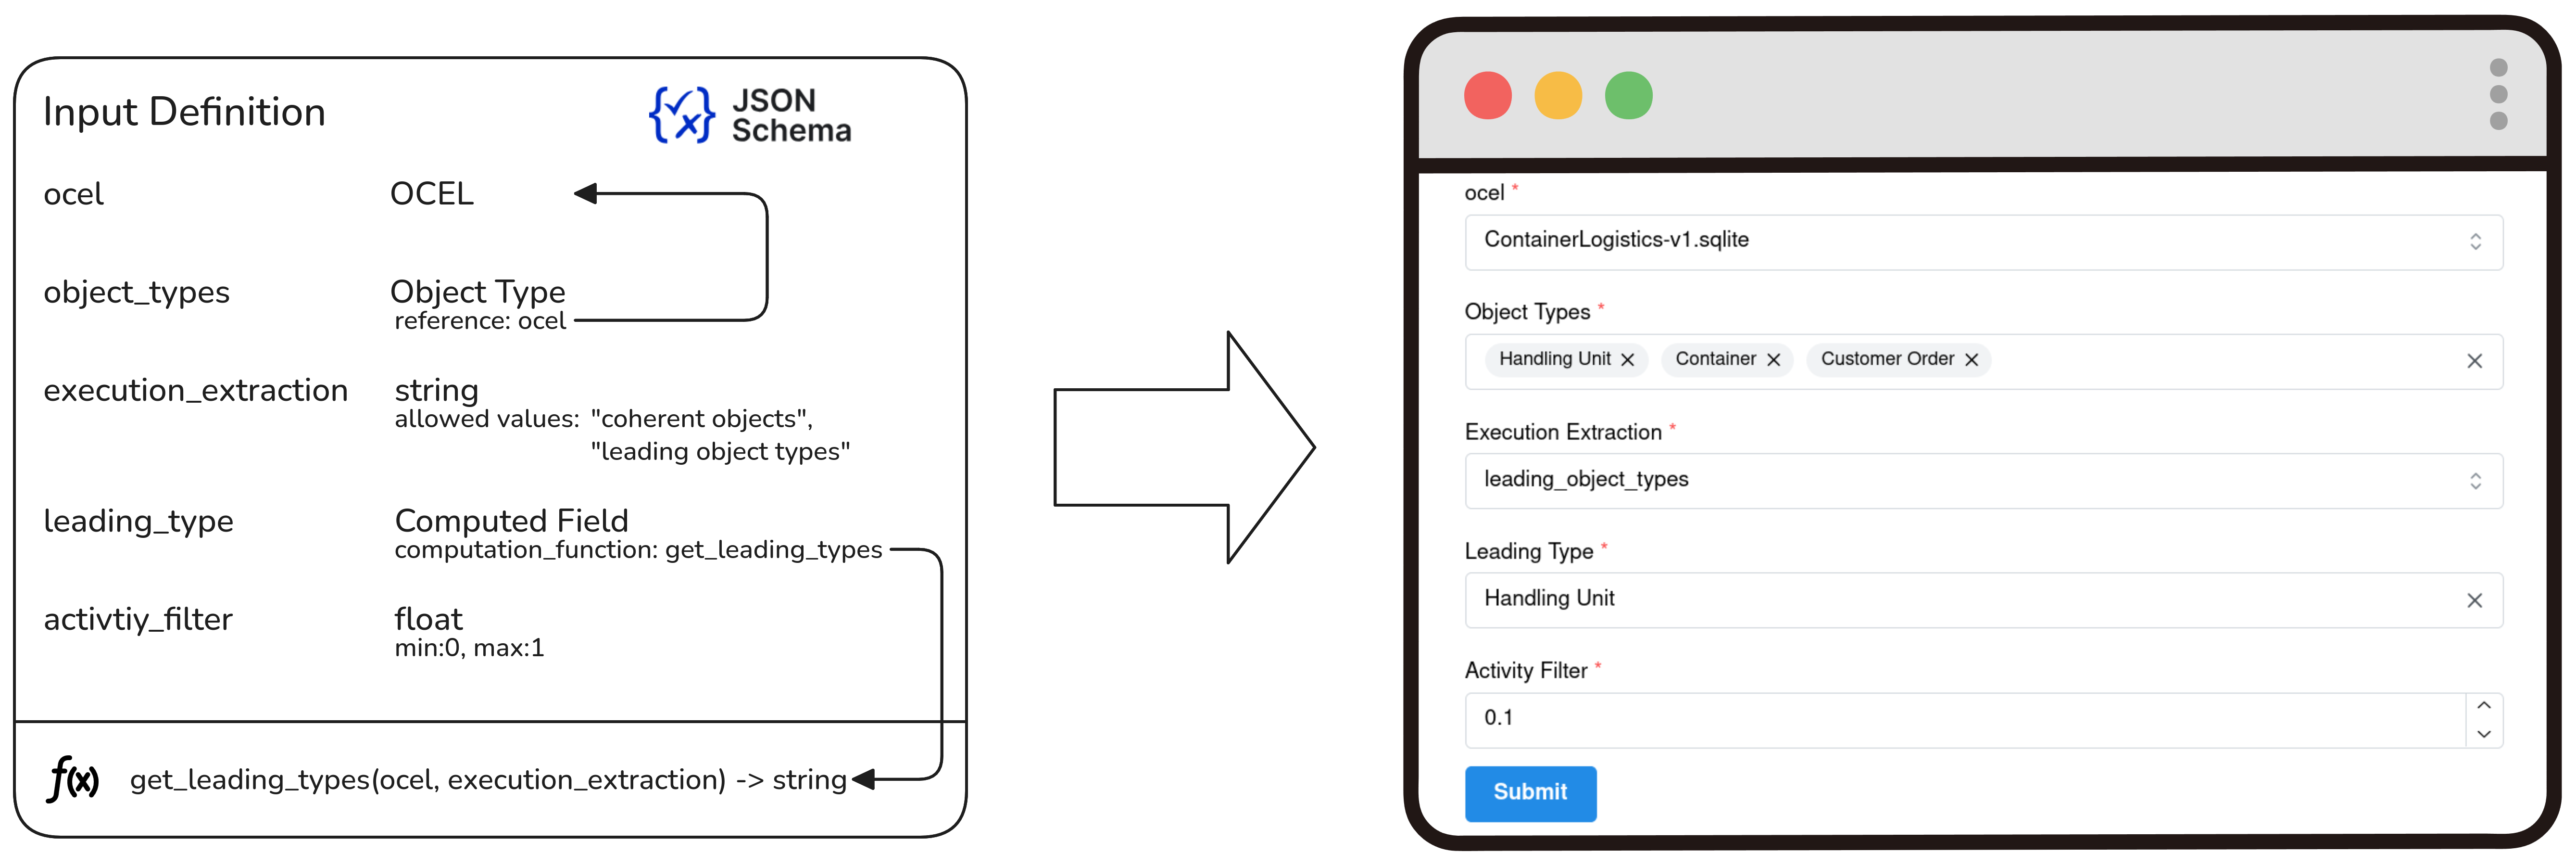
\includegraphics[width=\textwidth]{figures/design/Plugin Inputs.png}
	\caption{Example of a plugin input definition and the automatically generated input user interface.}
	\label{fig:plugin-inputs}
\end{figure}

\subsubsection{Functions and Executions}

Plugin functions are implemented in Python and are invoked by the backend using the input values submitted through the plugin interface. The input form produces a JSON object, which is passed to the corresponding function as its input. A plugin function can return OCEL instances or resource instances.

All outputs produced by a plugin function are stored in the session. The plugin interface then visualizes the resulting resources, allowing users to inspect the results directly in the frontend.

\begin{figure}[ht]
	\centering
	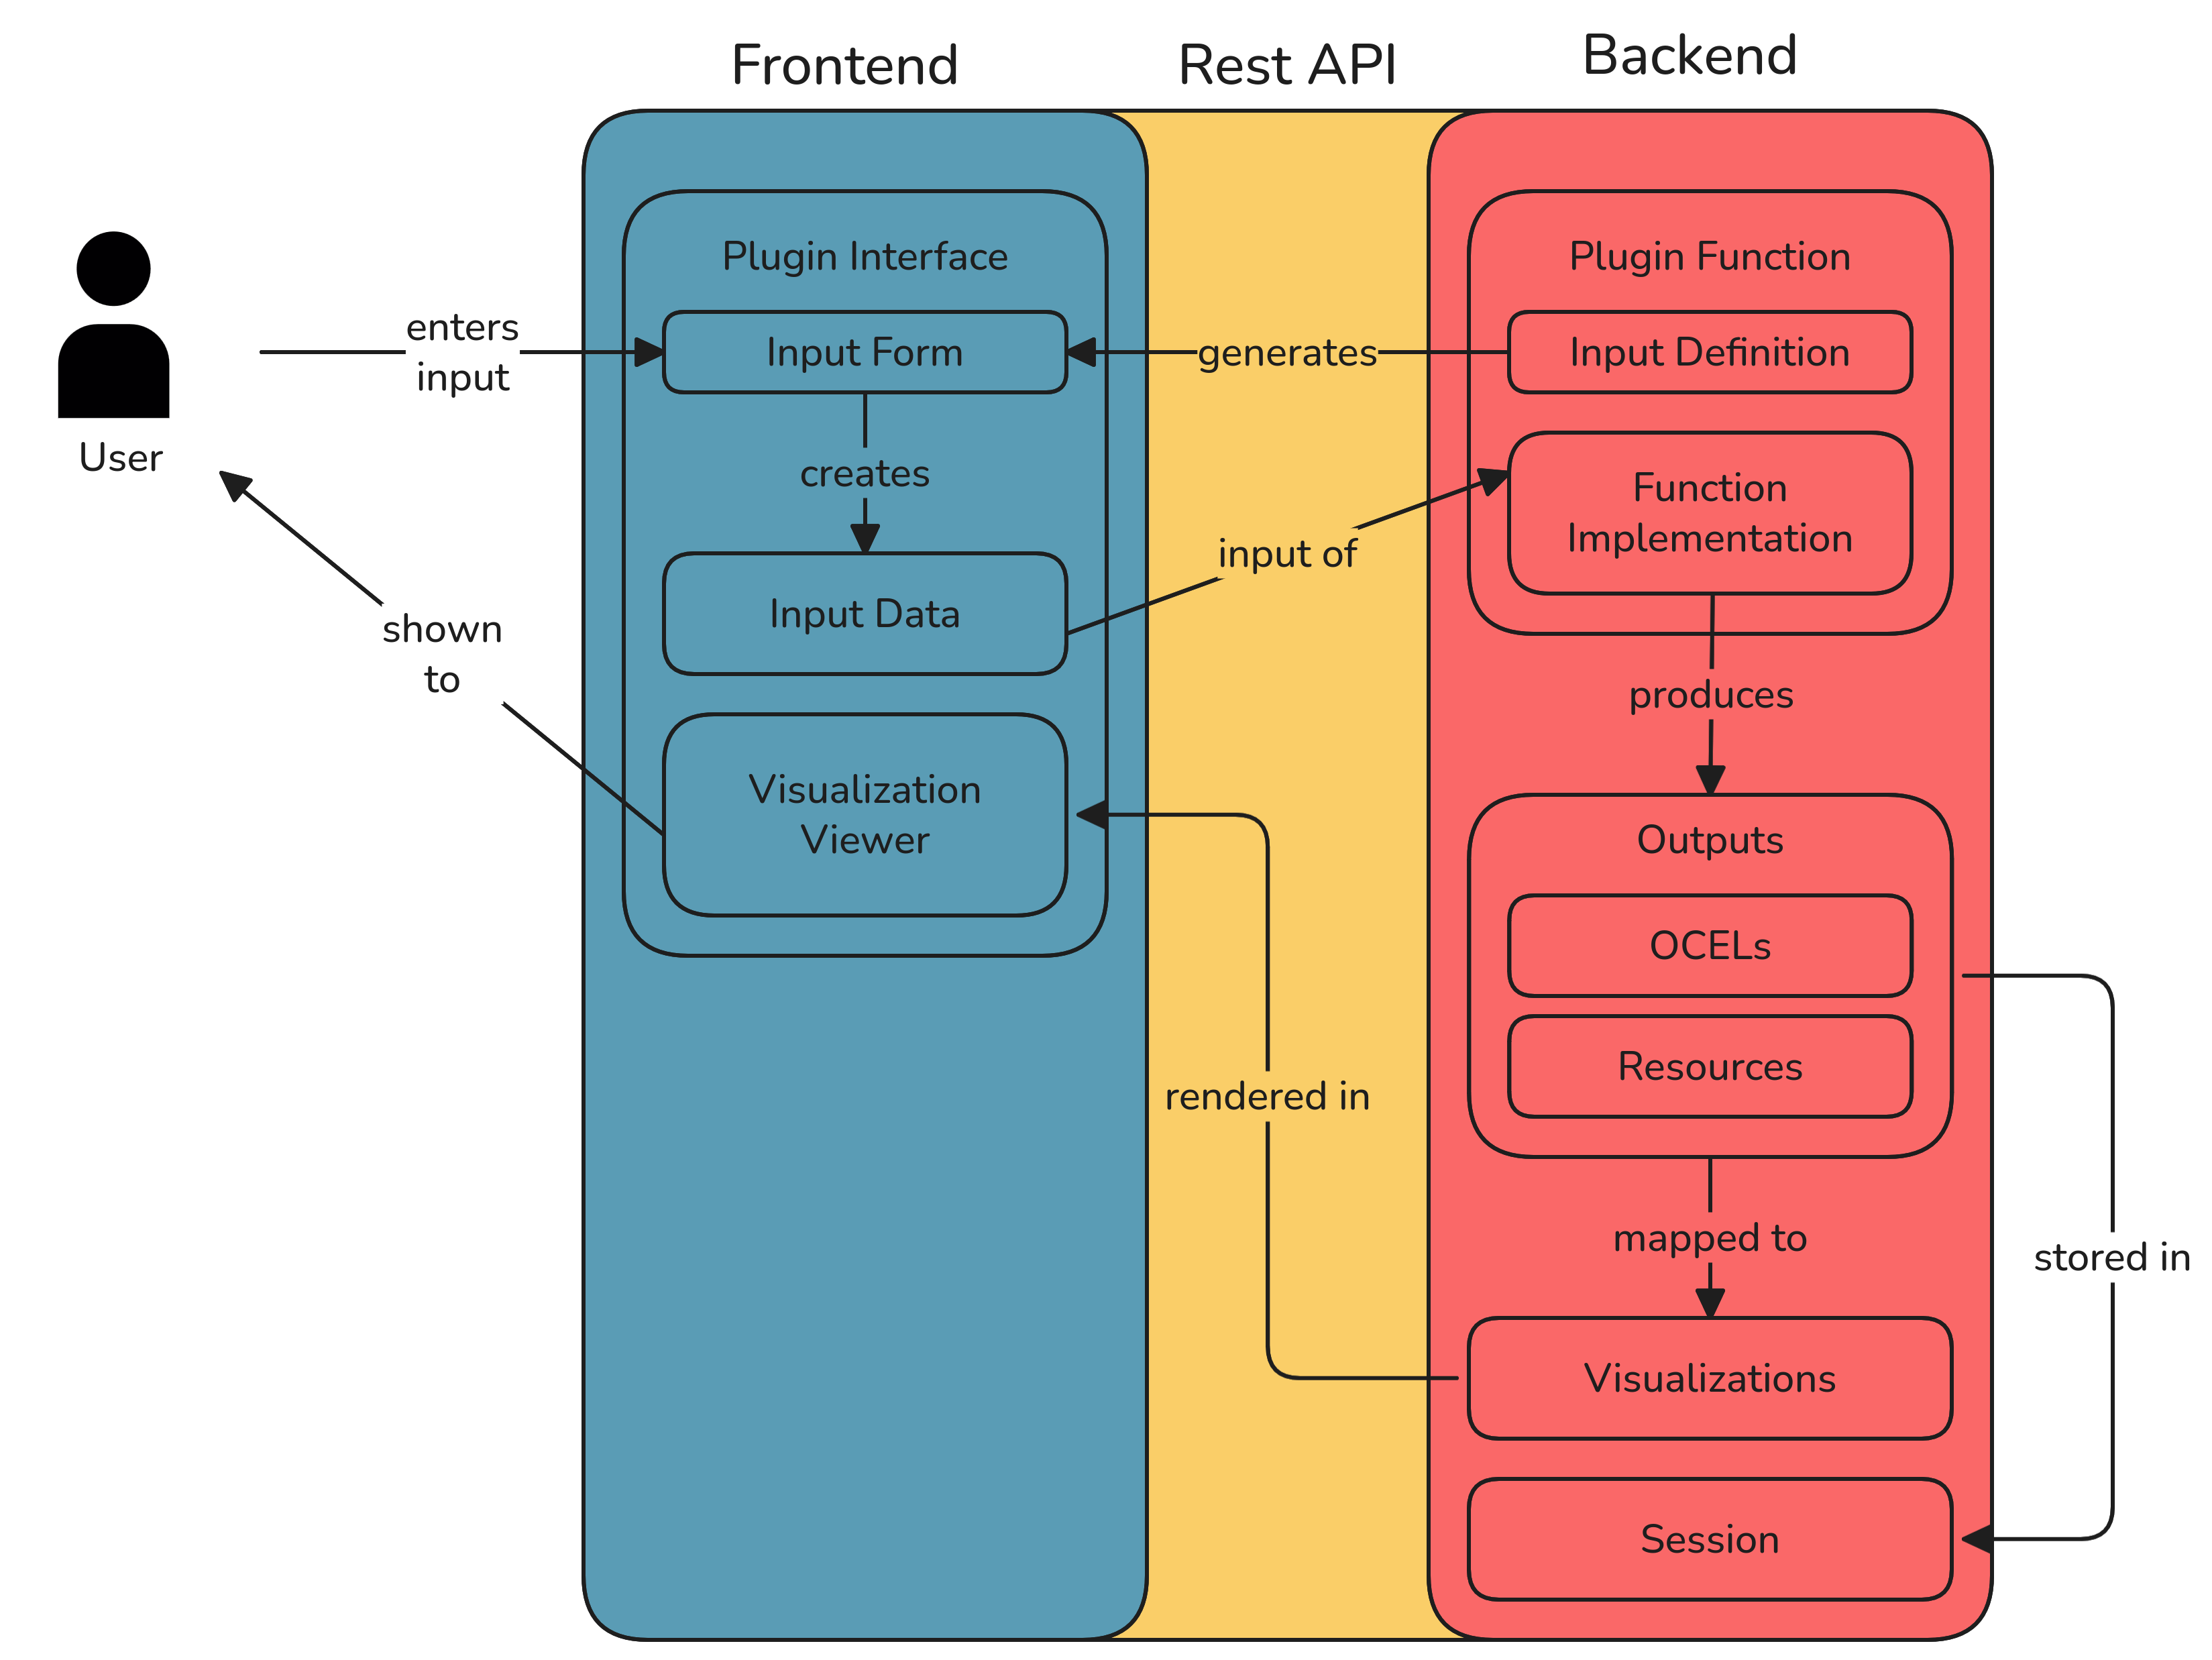
\includegraphics[width=0.5\textwidth]{figures/design/function_run.png}
	\caption{Overview of the execution of plugin functions. The frontend creates the input data, which is sent to the backend. The function processes the input and produces OCELs or resources. These outputs are stored in the session and visualized in the frontend.}
	\label{fig:function-execution}
\end{figure}

\section{Module Architecture}
Modules extend \textit{Ocelescope} beyond the capabilities of the plugin mechanism.
They address two main use cases that require more flexibility than plugins can provide.

The first use case concerns applications that do not fit the input output paradigm of plugins or that require specialized user interfaces and multi step interaction workflows.
An example of this is \textit{Ocelot}, where the main purpose of the tool is inspection rather than the production of new output.
Another example is constraint-based OCPM tools that use specialized graphical constraint builders~\cite{ocpq, proact, constraintchecking}.

The second use case targets tools intended for users who are not experts in process mining.
Users outside the domain may struggle to work with the plugin mechanism and automatically generated input fields.
Modules address this issue by providing domain-specific user interfaces that guide users through the analysis process.

For example, the \textit{OCEAn} tool~\cite{ocean} supports the definition of rules that enrich OCELs with sustainability data. These rules are defined by domain experts from the industry in which the OCELs originate. By enabling tailored user interfaces, modules allow such experts to enrich OCELs without requiring knowledge of OCPM.
To address these requirements, \textit{Ocelescope} provides \textbf{modules} as a second extension mechanism.
Modules are larger and self contained components that are built directly on top of the framework.

Two types of modules are supported:
\begin{itemize}
	\item \textbf{Frontend modules} for defining custom user interfaces, and
	\item \textbf{Backend modules} for extending the process mining functionality of the framework.
\end{itemize}

Frontend modules follow the microfrontend architecture and backend modules follow the microservice architecture, as introduced in \cref{chap:prelim}.
Both architectural patterns allow user interfaces and services to be developed as isolated, reusable units using established frameworks and therefore address \req{EM-3a}, \req{EM-3b}, and \req{EM-4a}.

\subsection{Frontend Modules.}

Frontend modules are based on the concept of \textit{microfrontends}~\cite{plugin-microservice}. Microfrontend architectures involve several key design decisions~\cite{microfrontends}:

\begin{itemize}
	\item \textbf{Split strategy:} Determines whether multiple modules can be shown at the same time.
	\item \textbf{Composition side:} Defines how modules are integrated into the main application.
	\item \textbf{Routing:} Specifies how navigation between modules is handled.
	\item \textbf{Communication:} Describes how modules exchange data or share state.
\end{itemize}

These design decisions are guided by two main goals. Frontend modules should be as independent as possible so that they can be reused or integrated into other applications with minimal effort. At the same time, they should integrate naturally into the overall interface so that the application remains cohesive.

\begin{figure}[ht]
	\centering
	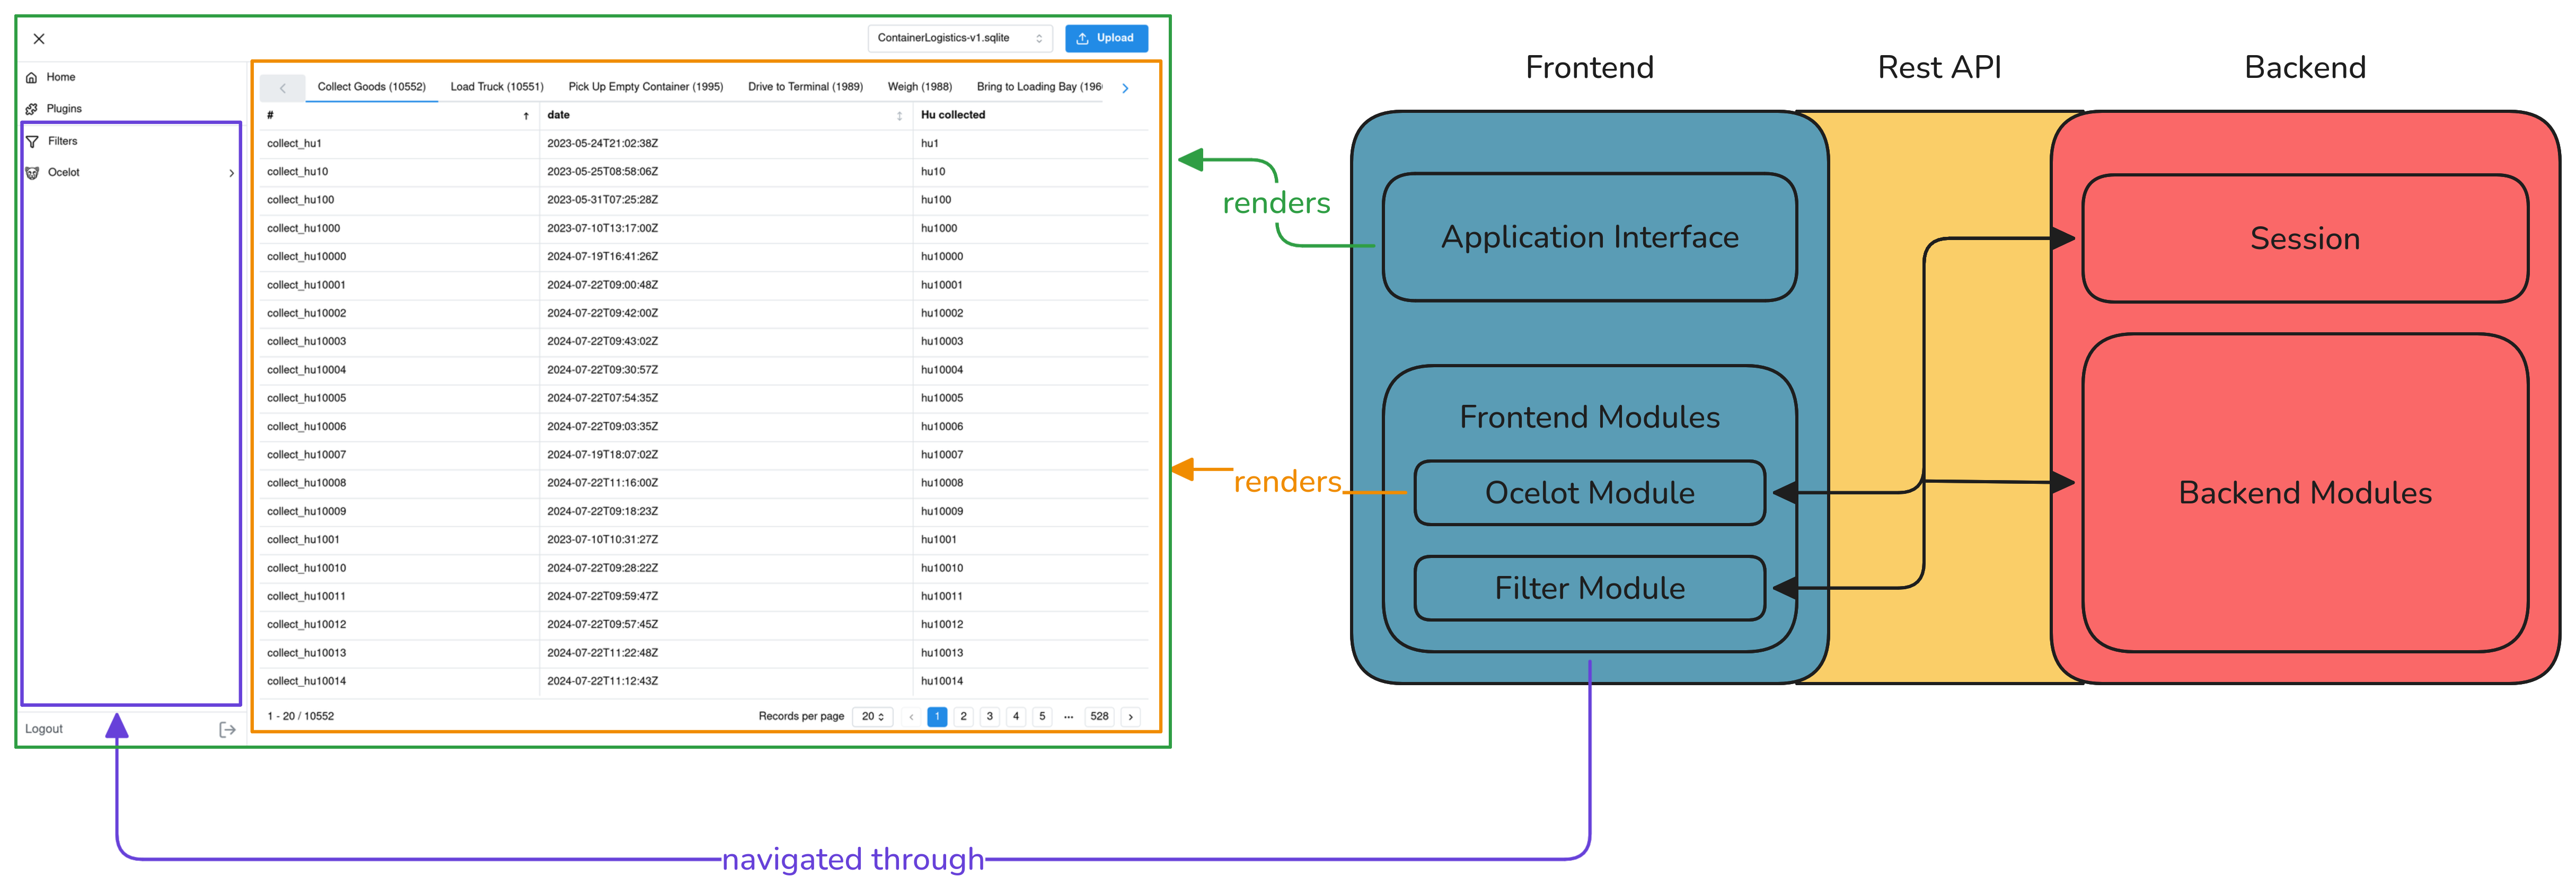
\includegraphics[width=\textwidth]{figures/design/FrontendModules.png}
	\caption{Frontend modules in \textit{Ocelescope}. The application shell renders module views and provides navigation. Each module is implemented as an independent microfrontend that integrates into the interface while sharing access to the session and backend modules.}
	\label{fig:frontend-modules}
\end{figure}

\textit{Ocelescope} adopts a \textbf{vertical split}. Each module is presented as a separate view within a shared application shell. The shell is responsible for navigation and ensures that the application appears as a unified system. Modules do not communicate directly with each other. Instead, they share access to the active sessions and can invoke backend modules when required. Each module may define one or more views, which are registered at build time and appear in the navigation panel.

\subsection{Backend Modules}

Backend modules follow the architectural principles of microservices and complement the microfrontend structure of the system. While frontend modules handle visualization and user interaction, backend modules implement independent process mining logic.

Unlike traditional microservices, which run as separate applications, backend modules in \textit{Ocelescope} are integrated into a shared backend environment. This avoids repeated loading of OCELs. Since all modules operate within the same backend, they can access OCEL instances that are already part of the session. Without this integration, each module would need to load the log again for every request, which would be inefficient.

Backend modules can also maintain their own state, which is useful for functionality that spans multiple requests. One example is object-centric process simulation~\cite{ocpsm}, where users step through a simulated execution and the simulation state must be preserved between calls. Modules state are stored within the user session.

Backend modules communicate with the frontend through REST API subroutes. They have access to the active session and can read or modify its content. Similar to frontend modules, backend modules are isolated from each other and can interact only through changes to the shared session.

\begin{figure}[ht]
	\centering
	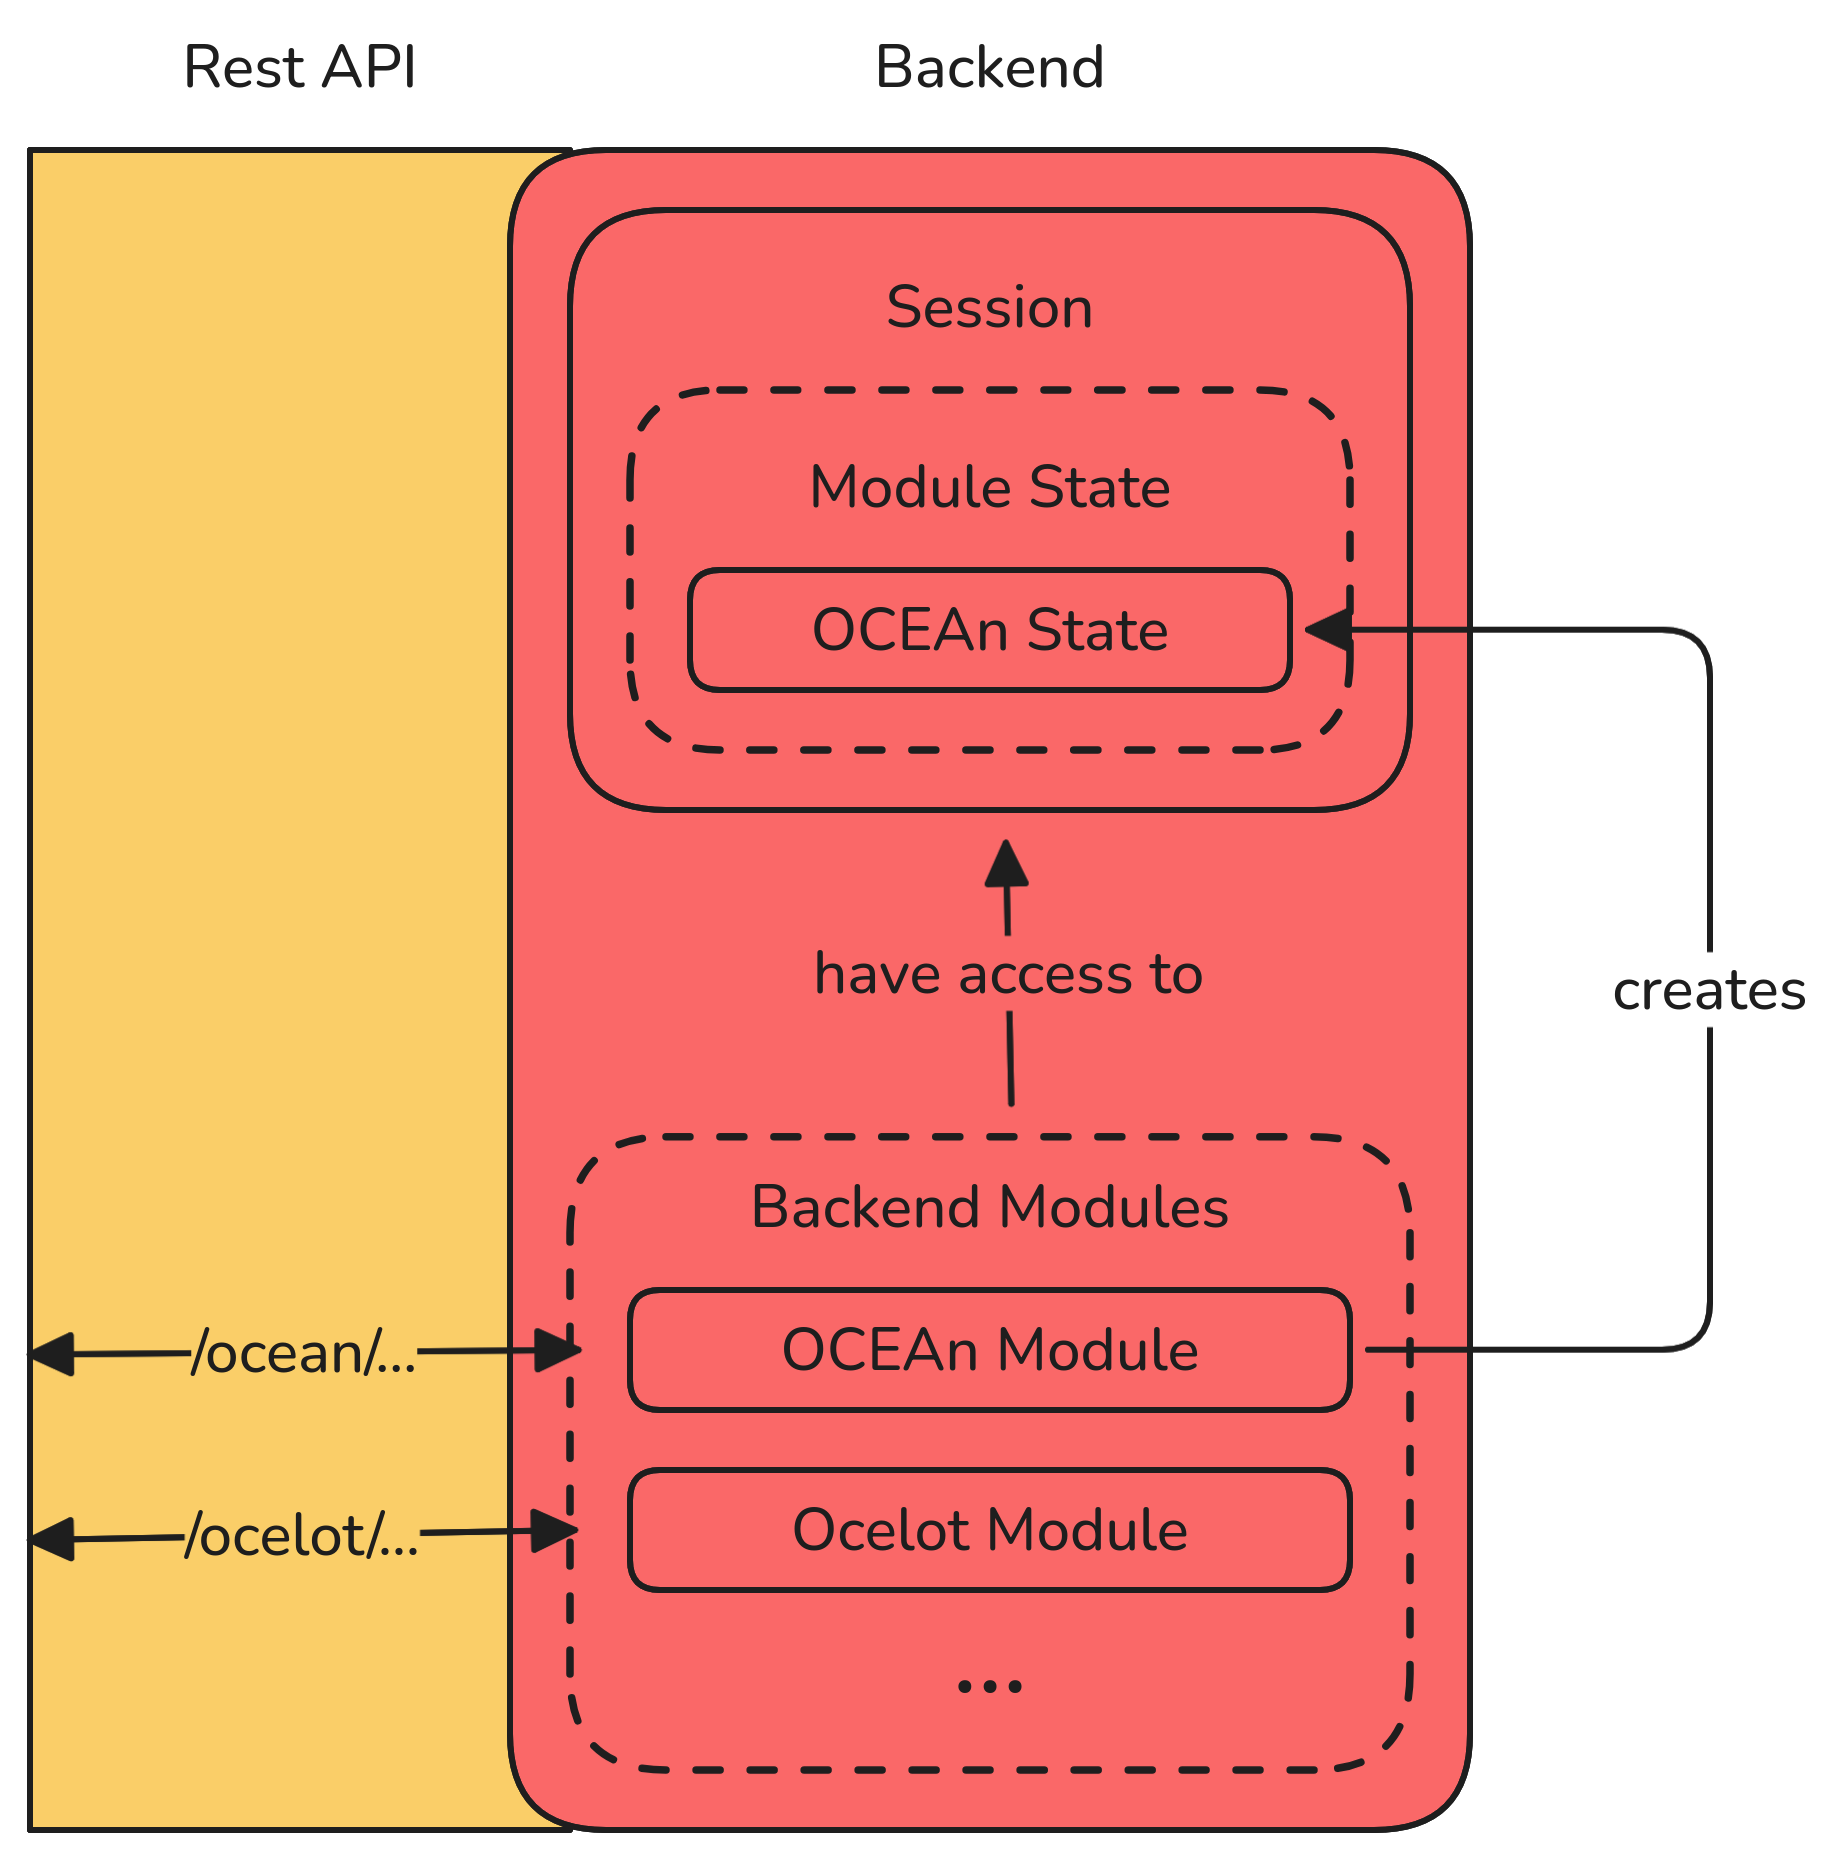
\includegraphics[width=0.35\textwidth]{figures/design/BackendModules.png}
	\caption{Backend modules in \textit{Ocelescope}. Modules expose REST API endpoints and access session data, including module-specific state. They operate independently while sharing access to active OCEL instances and updating the session state.}
	\label{fig:backend-modules}
\end{figure}

\subsection{Benefits of the Module Architecture}

Modules are integrated into \textit{Ocelescope} through an automated build process. They allow developers to focus on their main functionality and avoid writing boilerplate code or managing distribution. Tools that are built as modules benefit from the same protection against dependency rot and the same installation and deployment mechanisms as the main tool. This also encourages a modular design.

Both microfrontends and microservices share the goal of splitting complex applications into smaller and maintainable components \cite{plugin-microservice}. The module architecture in \textit{Ocelescope} follows this idea. It makes extensibility a central part of the framework rather than an afterthought. Developers can extend \textit{Ocelescope} without deep knowledge of its internal structure, because each module has a clear entry point and operates in isolation. This isolation improves maintainability and robustness. Bugs remain confined to individual modules, and new tools can be developed or updated independently.

\paragraph{Example based on \textit{ProAct}.}

To demonstrate the practical benefits of the module system, consider \textit{ProAct} \cite{proact}, a tool for evaluating business constraints. It was implemented as a standalone web application and is currently not operational due to dependency issues. Implementing it through the \textit{Ocelescope} module system would have prevented these issues. In addition, \textit{ProAct} would not need to reimplement boilerplate functionality such as OCEL management. As shown in \autoref{fig:module-example}, development could instead focus on its two main functionalities: process analysis, which visualizes performance metrics using an annotated directly follows graph, and constraint definition and evaluation via a graphical constraint builder. Implemented as modules, these functionalities could also be integrated into other OCPM applications built on \textit{Ocelescope}, for example by reusing the process analysis module to provide performance metrics.

\begin{figure}[ht]
	\centering
	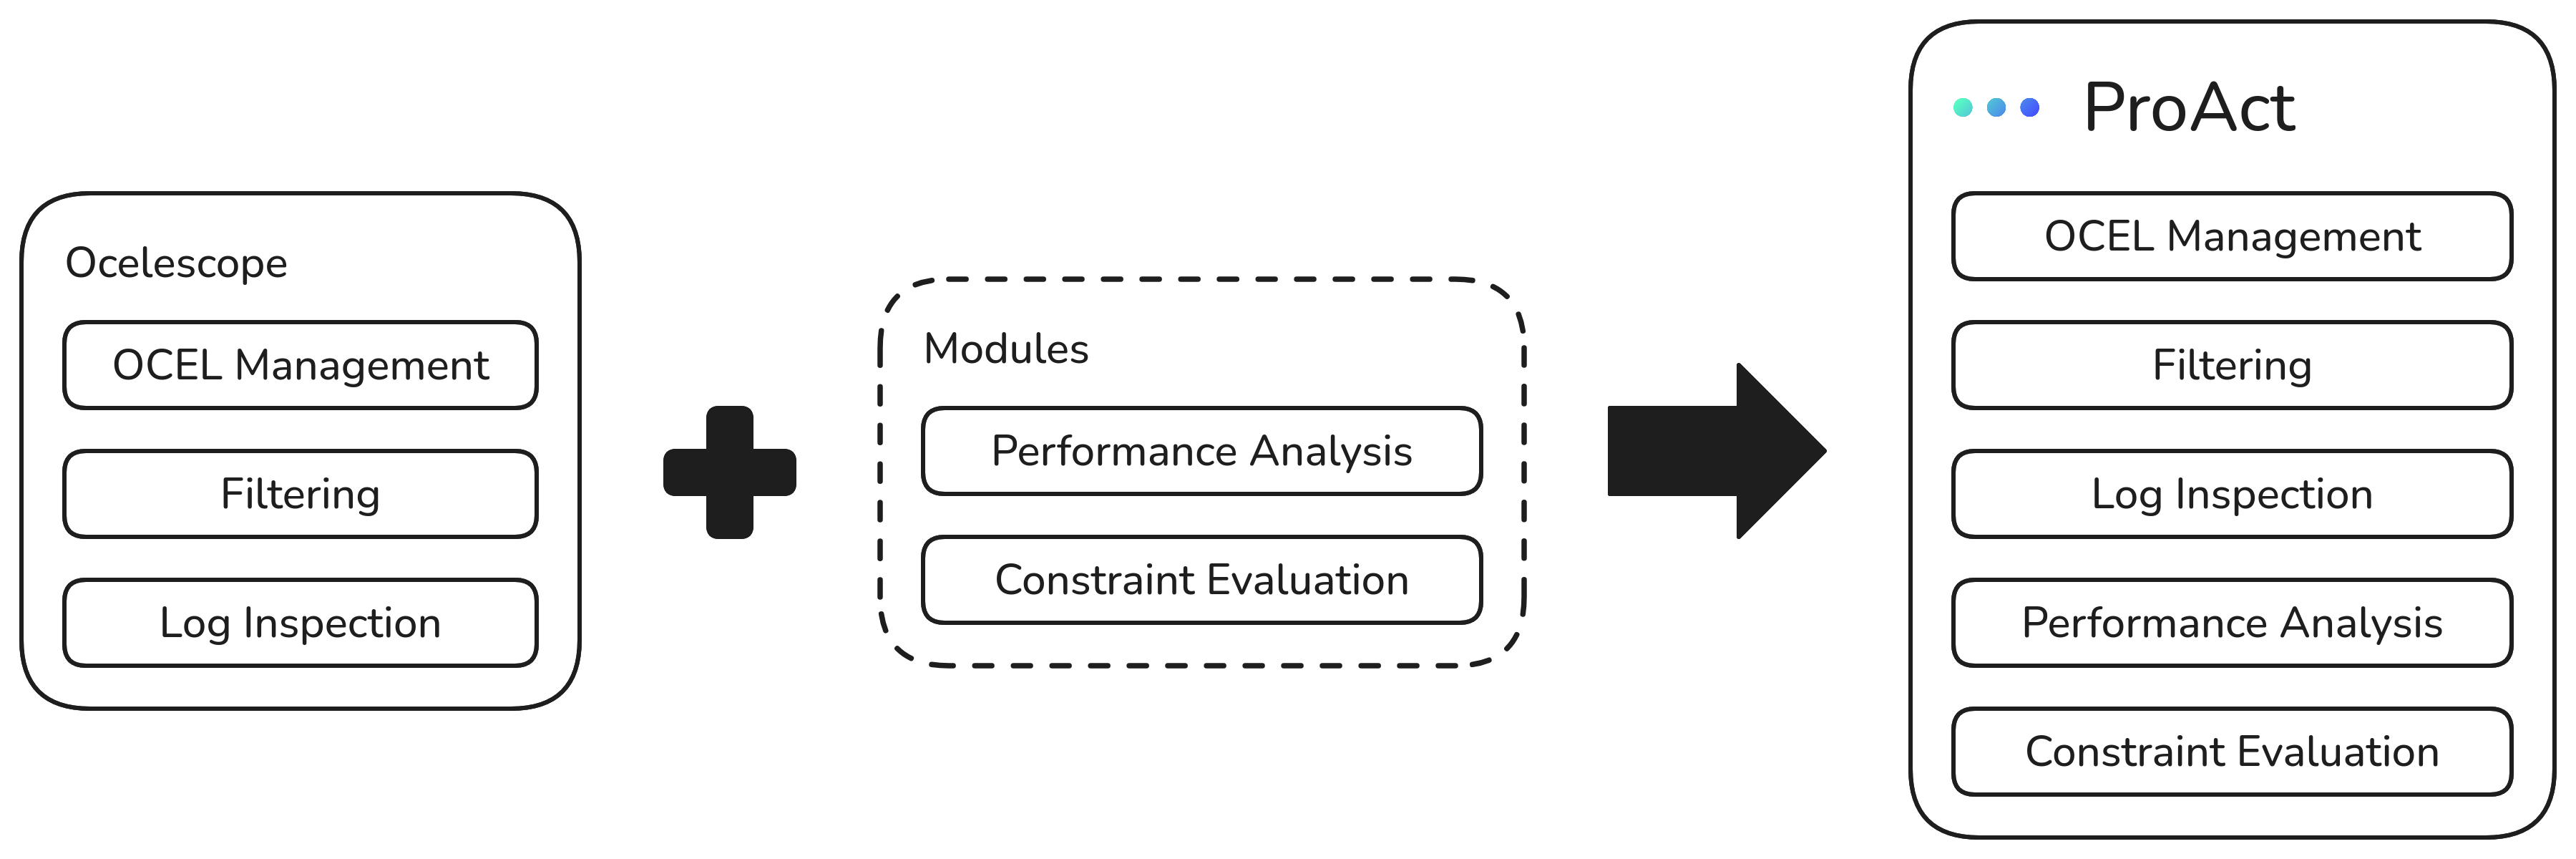
\includegraphics[width=\textwidth]{figures/design/ModuleExample.png}
	\caption{Example of how modules extend the base functionality of \textit{Ocelescope}.
		The core features of the framework, such as OCEL management, filtering, and log inspection, are combined with additional modules for performance analysis and constraint evaluation.
		Together these components form a complete application such as \textit{ProAct}.}
	\label{fig:module-example}
\end{figure}

\section{Containerization}

While the plugin and module architectures improve the extensibility of the \textit{Ocelescope} framework, extensibility alone is not sufficient if the framework cannot be installed reliably or maintained over time.
Requirements \req{BF-5a}, \req{BF-5b}, and \req{BF-5c} therefore emphasize robustness against dependency and versioning issues, minimal required system dependencies, and a simple setup process.
Research software often suffers from outdated dependencies, broken installations, or environments that cannot be reproduced~\cite{dockerinscience}.
To address these issues, \textit{Ocelescope} follows a containerization strategy similar to the one suggested in~\cite{dockerinscience}.

Both the frontend and the backend are distributed as container images that include all required dependencies (\req{BF-5b}).
This also covers system-level requirements because the images run in a controlled environment that provides a consistent execution context.
For example, \textit{oCoCoMot}~\cite{ococomot}, which depends on SMT solvers, can be included directly in a backend image.
This encapsulates the required setup steps and ensures consistent behavior across different machines.

Container images are built, versioned, and stored in a container image registry.
Running \textit{Ocelescope} requires only a container engine such as Docker, which provides lightweight virtualization across all major operating systems and is easy to install.
With the help of start scripts, the tool can be launched using a single command (\req{BF-5c}).

Versioned container images provide an additional benefit for long-term robustness.
Each plugin or module is associated with a specific environment in which it is known to function correctly (\req{BF-5a}), since the environment is already built and preserved in the registry.
Deployment as a web application is also simplified, as many hosting providers support running container images directly, and self-hosted deployments are equally possible.

\begin{figure}[ht]
	\centering
	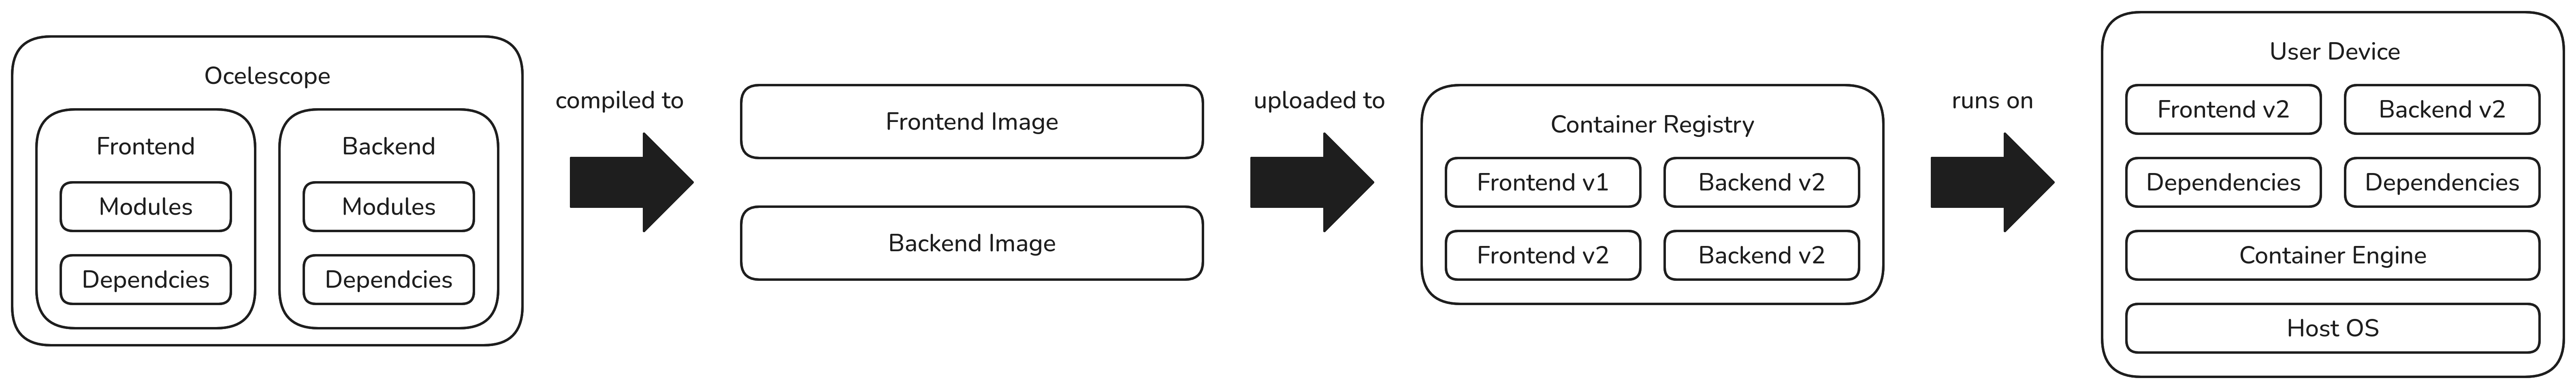
\includegraphics[width=\textwidth]{figures/design/ContainerExample.png}
	\caption{Containerization workflow in \textit{Ocelescope}. The frontend and backend, together with all modules and dependencies, are packaged into container images and stored in a registry. Users can run specific versions on different systems using a container engine, which provides a consistent and reproducible execution environment.}
	\label{fig:container-example}
\end{figure}

\section{Filtering}
\label{sec:filtering}

Filtering is an essential step in most OCPM tools and is therefore a basic requirement of the framework (\req{BF-3a}).
\textit{Ocelescope} therefore provides a set of basic filters. Many filters used in existing tools focus on basic properties, such as filtering by activity types~\cite{ocpi} or by relation counts~\cite{oxminer}. The filtering functions in \textit{Ocelescope} follow the structure of the \textit{OCEL~2.0} metamodel and cover the most common properties of events and objects. They are designed to be easy to use and do not require knowledge of a query language.

More specialized filtering can be implemented within a plugin function or as a separate module, particularly when a custom user interface is beneficial. One example is the query language of \textit{OCPQ}~\cite{ocpq}, which relies on a dedicated interface.

\textit{Ocelescope} supports the following filtering functionality:

\begin{itemize}
	\item \textbf{Filtering by type:}
	      Events and objects can be selected based on their assigned types. For events, this corresponds to selecting activity names, and for objects, it corresponds to selecting object types.

	\item \textbf{Filtering by timestamp:}
	      Events can be restricted to a user-defined time window. Only events whose timestamps lie within the selected range are retained.

	\item \textbf{Filtering by attribute values:}
	      Events and objects contain additional attributes that can be used for filtering. Conditions can be defined on attribute names and values. Supported value types include:
	      \begin{itemize}
		      \item \textbf{Strings:} selection by lists of values or regular expressions,
		      \item \textbf{Numbers:} selection by numeric ranges,
		      \item \textbf{Dates:} selection by date or time ranges.
	      \end{itemize}

	\item \textbf{Filtering by relation counts:}
	      Entities can be filtered based on the number of event-to-object (E2O) or object-to-object (O2O) relations they have to entities of a specified type. A relation qualifier can also be taken into account.
\end{itemize}

\begin{figure}[ht]
	\centering
	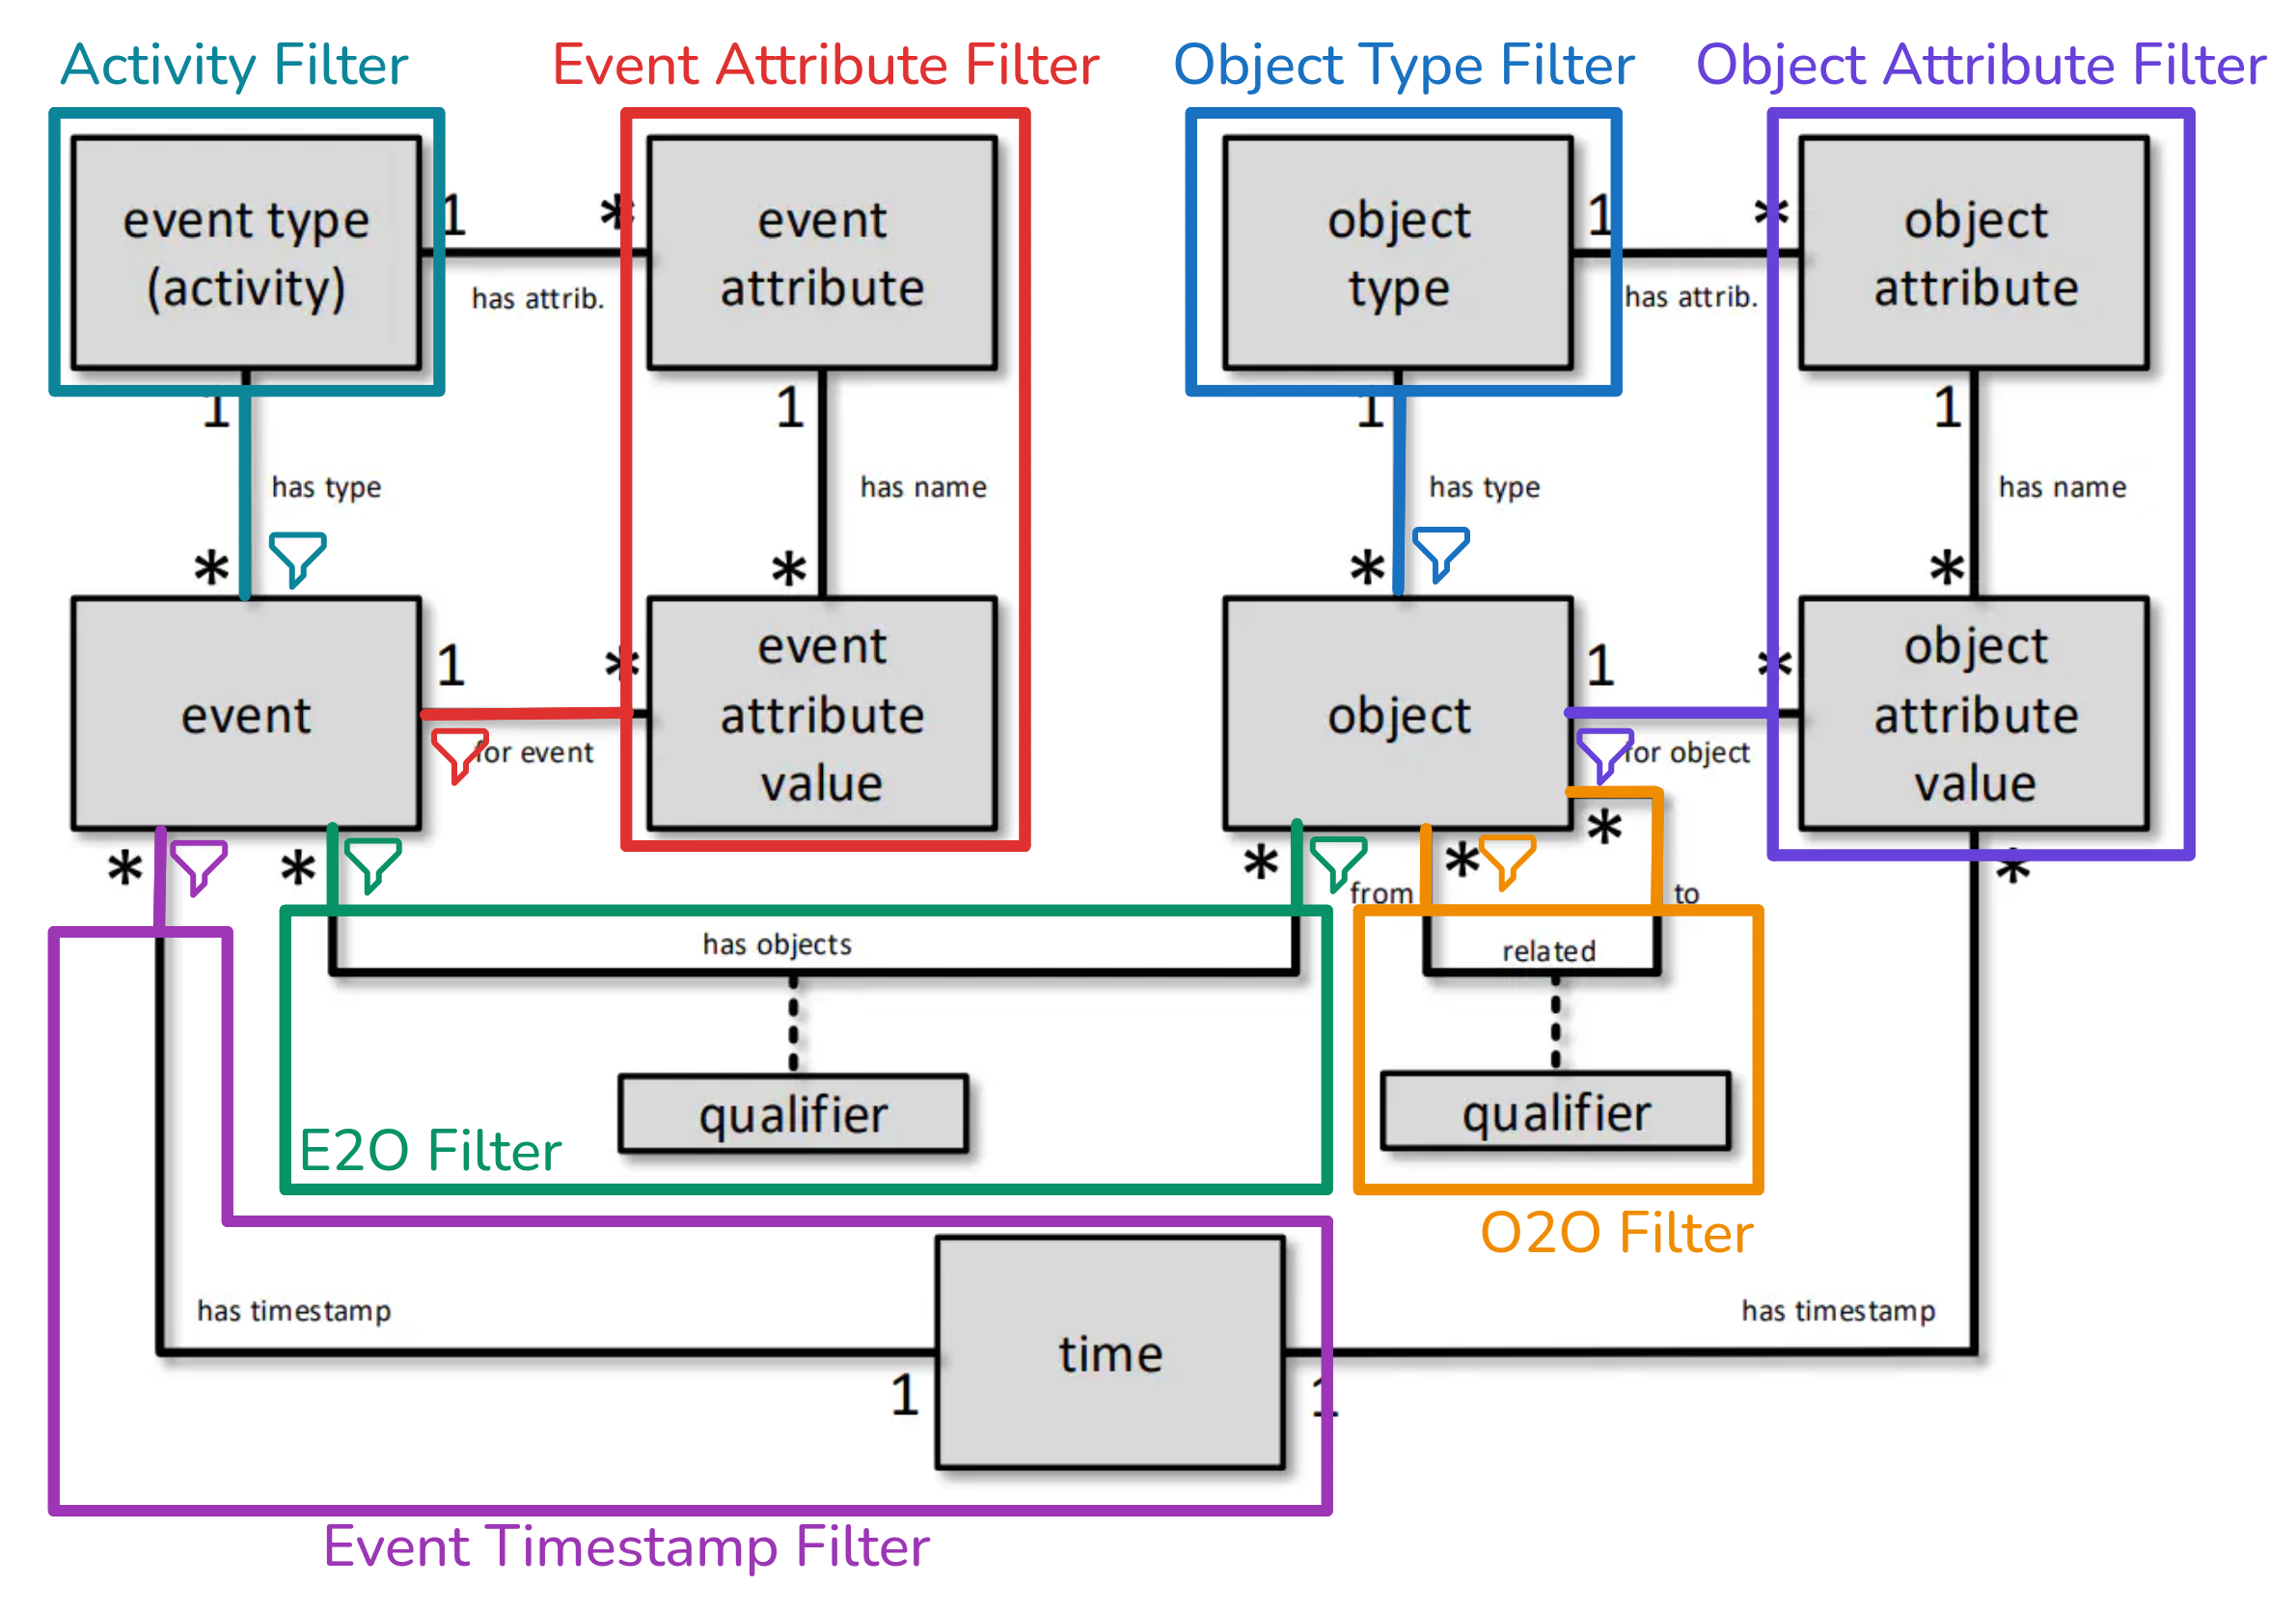
\includegraphics[width=0.6\textwidth]{figures/design/FilterInMetaModel.png}

	\caption{Filtering operations in \textit{Ocelescope} shown in relation to the OCEL 2.0 metamodel.
	}
	\label{fig:filter-metamodel}
\end{figure}
